\section{Projections}
Given our current project state, we have revised our schedule as follows:
\begin{figure}[h!]
  \centering
  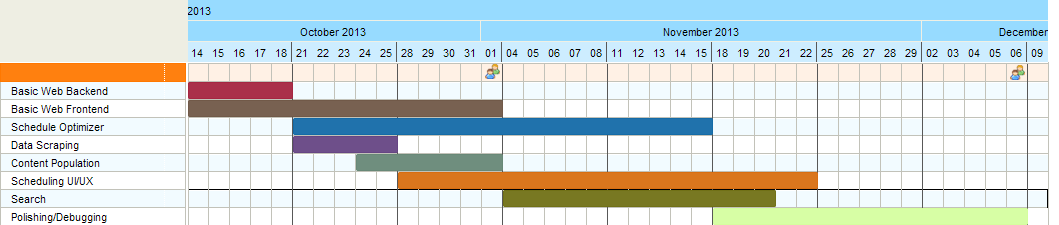
\includegraphics[width=\textwidth]{gantt.png}
  \caption{Original Gantt chart demonstrating proposed project schedule}
\end{figure}
\begin{figure}[h!]
  \centering
  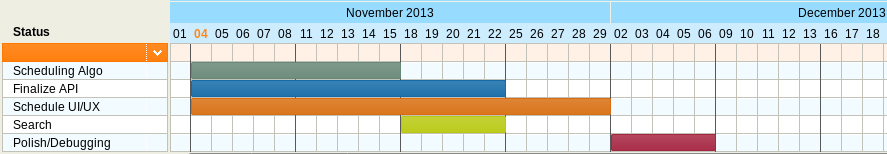
\includegraphics[width=\textwidth]{revised-gantt.png}
  \caption{Revised Gantt chart for next month}
\end{figure}

As demonstrated in our revised chart and as discussed previously, we have
completed the basic components of both the front and backend. We have also
made enough progress on the data scraping so that we can summarize the
remaining backend work as finalizing the API. Thanks to the time initially
allocated to getting the schedule optimizer working, the backend team is
currently slightly ahead of schedule. We believe this is positive, as it will
give them an opportunity to create the best possible scheduling algorithm.

Our frontend has significantly more to do: although the frontend group
has completed the basics, there still exists considerable work required
before the user-facing site and user experience (UX) will be complete.
The frontend team is currently on-schedule to finish as expected initially,
and will hopefully be able to pull ahead of schedule as work on the UI
progresses.

Beyond this, the backend and frontend teams will then collaborate to create
the planned search feature. The final week is reserved for polishing and
debugging the site, giving us time to test and make sure everything is perfect
before we release it to the public.
